\documentclass{article}
\usepackage[margin=1in]{geometry}
\usepackage{problemset}
\showsolntrue

% Custom commands
\newcommand{\R}{\mathbb{R}}
\newcommand{\X}{\mathcal{X}}
\newcommand{\Y}{\mathcal{Y}}
\newcommand{\E}{\mathbb{E}}
\newcommand{\V}{\text{Var}}
\renewcommand{\P}{\mathbb{P}}

\begin{document}

\pstitle{%
    MATH 181A%
}{
    Homework 8%
}[due Thursday, March 5 at 11:59PM]

\begin{probset}
% --- Problem 1 ---
\begin{prob}[\textbf{7.4.12}]
    If a normally distributed sample of size $n = 16$ produces a 95\% confidence interval for $\mu$ that ranges from 44.7 to 49.9, what are the values of $\bar{y}$ and $s$?

    \begin{soln}
        Since the interval is symmetric about $\bar{y}$, we have $\bar{y} = \frac{44.7 + 49.9}{2} = 47.3$. For $n = 16$ with unknown $\sigma$, we use the $t$-distribution: $t_{0.025, 15} \approx 2.131$. The radius of the interval is given by 
        \[
            2.131 \frac{s}{\sqrt{16}} = \frac{49.9 - 44.7}{2} = 2.6 \implies s = \frac{2.6 \cdot 4}{2.131} \approx 4.88
        \]
    \end{soln}
\end{prob}

\newpage

% --- Problem 2 ---
\begin{prob}[\textbf{7.4.20}]
    Make the decision in two ways using the
    t-table in Appendix A.2: (1) finding the critical region; and (2) finding the range of the p-value. 
    
    \textbf{Note:} the sample mean and sample standard deviation of the 34 ratios in the table are $0.6373$ and $0.14139$ respectively.
    
    In addition to the Shoshoni data of Case Study 7.4.2, a set of rectangles that might tend to the golden ratio are national flags. The table below gives the width-to-length ratios for a random sample of the flags of thirty-four countries. Let $\mu$ be the width-to-length ratio for national flags. At the $\alpha = 0.01$ level, test $H_0 : \mu = 0.618$ versus $H_1 : \mu \neq 0.618$.

    \begin{center}
        \begin{tabular}{cccc}
            \hline
            Country & Ratio Width to Height & Country & Ratio Width to Height \\
            \hline
            Afghanistan & 0.500 & Iceland & 0.720 \\
            Albania & 0.714 & Iran & 0.571 \\
            Algeria & 0.667 & Israel & 0.727 \\
            Angola & 0.667 & Laos & 0.667 \\
            Argentina & 0.667 & Lebanon & 0.667 \\
            Bahamas & 0.500 & Liberia & 0.526 \\
            Denmark & 0.757 & Macedonia & 0.500 \\
            Djibouti & 0.553 & Mexico & 0.571 \\
            Ecuador & 0.500 & Monaco & 0.800 \\
            Egypt & 0.667 & Namibia & 0.667 \\
            El Salvador & 0.600 & Nepal & 1.250 \\
            Estonia & 0.667 & Romania & 0.667 \\
            Ethiopia & 0.500 & Rwanda & 0.667 \\
            Gabon & 0.750 & South Africa & 0.667 \\
            Fiji & 0.500 & St. Helena & 0.500 \\
            France & 0.667 & Sweden & 0.625 \\
            Honduras & 0.500 & United Kingdom & 0.500 \\
            \hline
        \end{tabular}
    \end{center}
    \textit{Data from: http://www.anyflag.com/country/costaric.php}

    \begin{subprobset}
    \begin{subprob}
        Finding the critical region.

        \begin{soln}
            The critical region is when $|t| > t_{0.005}$ where $t_{0.005}$ is found from the (df=33, 0.005) entry of the t-table. We find that $t_{0.005} = 2.7333$. Hence, the critical region is when $|t| > 2.7333$. Our t-statistic is given by
            \[
                t = \frac{\bar{y} - \mu_0}{s/\sqrt{n}} = \frac{0.6373 - 0.618}{0.14139/\sqrt{34}} = 0.7959
            \]
            Since $|0.7959| < 2.7333$, we fail to reject $H_0$.
        \end{soln}
    \end{subprob}

    \begin{subprob}
        Finding the range of the p-value.

        \begin{soln}
            Using our previously calculated t-statistic, we can see in the t-table that a t-statistic of 0.7959 has greater p-value than 0.20 (the largest p-value in the table) which has a statistic of 0.8527. Hence, $p > 2 \cdot 0.20 = 0.40 > \alpha = 0.01$, so we fail to reject $H_0$.
        \end{soln}
    \end{subprob}
    \end{subprobset}
\end{prob}

\newpage

% --- Problem 3 ---
\begin{prob}[\textbf{7.4.21}]
    Make the decision in two ways using the t-table in Appendix A.2: (1) finding the critical region; and (2) finding the range of the p-value.
    
    A manufacturer of pipe for laying underground electrical cables is concerned about the pipe's rate of corrosion and whether a special coating may retard that rate. As a way of measuring corrosion, the manufacturer examines a short length of pipe and records the depth of the maximum pit. The manufacturer's tests have shown that in a year's time in the particular kind of soil the manufacturer must deal with, the average depth of the maximum pit in a foot of pipe is 0.0042 inch. To see whether that average can be reduced, ten pipes are coated with a new plastic and buried in the same soil. After one year, the following maximum pit depths are recorded (in inches): 0.0039, 0.0041, 0.0038, 0.0044, 0.0040, 0.0036, 0.0034, 0.0036, 0.0046, and 0.0036. Given that the sample standard deviation for these ten measurements is 0.000383 inch, can it be concluded at the $\alpha = 0.05$ level of significance that the plastic coating is beneficial?

    \begin{subprobset}
    \begin{subprob}
        Finding the critical region.
        
        \begin{soln}
            The critical region is when $t < -t_{0.05}$ where $t_{0.05}$ is found from the (df=9, 0.05) entry of the t-table. We find that $t_{0.05} = 1.8331$. Hence, the critical region is when $t < -1.8331$. Our t-statistic is given by
            \[
                t = \frac{\bar{y} - \mu_0}{s/\sqrt{n}} = \frac{0.0039 - 0.0042}{0.000383/\sqrt{10}} = -2.4770
            \]
            Since $-2.4770 < -1.8331$, we reject $H_0$.
        \end{soln}
    \end{subprob}

    \begin{subprob}
        Finding the range of the p-value.

        \begin{soln}
            Using our previously calculated t-statistic, we can see in the t-table that a t-statistic of $-2.4770 \in (2.2622, 2.821)$ which are p-values of 0.025 and 0.01 respectively. Hence, $p \in (0.01, 0.025) < \alpha = 0.05$, so we reject $H_0$.
        \end{soln}
    \end{subprob}
    \end{subprobset}
\end{prob}

% --- Problem 4 ---
\begin{prob}[\textbf{7.5.8}]
    A random sample of size $n = 19$ is drawn from a normal distribution for which $\sigma^2 = 12.0$. In what range are we likely to find the sample variance, $s^2$? Answer the question by finding two numbers $a$ and $b$ such that 
    $$P(a \leq S^2 \leq b) = 0.95$$

    \begin{soln}
        We use the fact that $(n-1)S^2/\sigma^2 \sim \chi^2_{n-1}$. With $n = 19$ and $\sigma^2 = 12$, we have $\frac{18S^2}{12} \sim \chi^2_{18}$. For a 95\% central interval, we need $P(\chi^2_{0.025,18} \leq \frac{18S^2}{12} \leq \chi^2_{0.975,18}) = 0.95$. From the chi-squared table: $\chi^2_{0.025,18} \approx 8.23$ and $\chi^2_{0.975,18} \approx 31.53$. Hence
        \[
            a = \frac{8.23 \cdot 12}{18} \approx 5.49, \qquad b = \frac{31.53 \cdot 12}{18} \approx 21.02
        \]
    \end{soln}
\end{prob}

\newpage

% --- Problem 5 ---
\begin{prob}[\textbf{7.3.4}]
    Use the fact that $(n-1)S^2/\sigma^2$ is a chi square random variable with $n - 1$ df to prove that
    $$\V(S^2) = 2\sigma^4 / (n - 1)$$
    (\textit{Hint:} Use the fact that the variance of a chi square random variable with $k$ df is $2k$.)

    \begin{soln}
        We use the fact that $(n-1)S^2/\sigma^2 \sim \chi^2_{n-1}$. The variance of a chi-squared random variable with $k$ df is $2k$. Hence
        \[
            \V\left(\frac{(n-1) S^2}{\sigma^2}\right) = \left(\frac{n-1}{\sigma^2}\right)^2 \V(S^2) = 2(n-1) \implies \V(S^2) = \frac{2\sigma^4}{n-1}
        \]
    \end{soln}
\end{prob}

% --- Problem 6 ---
\begin{prob}[\textbf{7.3.10}]
    Suppose $X_1, \ldots, X_n$ are i.i.d. random variables having a $N (\mu, \sigma^2)$ distribution. Consider the estimator of $\sigma^2$,
    $$\hat{\sigma}^2_c = c \sum_{i=1}^n (X_i - \bar{X})^2$$
    Recall that $\hat{\sigma}^2_c$ is the MLE if $c = 1/n$ and is the unbiased estimator $S^2$ if $c = 1/(n - 1)$.

    \begin{subprobset}
    \begin{subprob}
        Calculate the mean squared error of $\hat{\sigma}^2_c$.

        \begin{soln}
            We have $\hat{\sigma}^2_c = c \sum_{i=1}^n (X_i - \bar{X})^2 = c(n-1)S^2$. We know that $\E[S^2] = \sigma^2$ and $\V(S^2) = 2\sigma^4/(n-1)$. We also know:
            \[
                \text{MSE}(\hat{\sigma}^2_c) = \V(\hat{\sigma}^2_c) + \bigl(\E[\hat{\sigma}^2_c] - \sigma^2\bigr)^2.
            \]

            $\E[\hat{\sigma}^2_c] = c(n-1)\E[S^2] = c(n-1)\sigma^2$, so $\text{Bias} = c(n-1)\sigma^2 - \sigma^2 = \sigma^2\bigl(c(n-1) - 1\bigr)$.

            $\V(\hat{\sigma}^2_c) = c^2(n-1)^2 \V(S^2) = c^2(n-1)^2 \cdot \frac{2\sigma^4}{n-1} = 2c^2(n-1)\sigma^4$.
            \[
                \text{MSE}(\hat{\sigma}^2_c) = 2c^2(n-1)\sigma^4 + \sigma^4\bigl(c(n-1) - 1\bigr)^2.
            \]
        \end{soln}
    \end{subprob}

    \begin{subprob}
        For which value of $c$ is the mean squared error the smallest?

        \begin{soln}
            We find the minimum MSE by taking the derivative of the MSE with respect to $c$ and setting it to 0.
            \begin{align*}
                \frac{d}{dc} \text{MSE}(\hat{\sigma}^2_c) = 4c(n-1)\sigma^4 + 2(n - 1)\sigma^4(c(n-1) - 1) &= 0 \\
                \implies 2c + nc - c - 1 &= 0 \\
                \implies c = \frac{1}{n + 1}
            \end{align*}
        \end{soln}
    \end{subprob}
    \end{subprobset}
\end{prob}

\newpage

% --- Problem 7 ---
\begin{prob}[\textbf{R Simulation}]
    Use 5000 repetitions to generate two empirical density functions in the same plot to verify

    \begin{subprobset}
    \begin{subprob}
        The empirical distribution of $X_1^2 + X_2^2 + \cdots + X_9^2$ (using a solid line) is close to that of $\chi^2_9$ (using a dashed line), where $X_i \sim \text{i.i.d.} N (0, 1)$.

        \begin{verbatim}
set.seed(42)
n_rep <- 5000

png("7a.png", width = 8, height = 5, units = "in", res = 150)  # landscape

empirical <- replicate(n_rep, sum(rnorm(9, 0, 1)^2))

theoretical <- rchisq(n_rep, df = 9)

dens_emp <- density(empirical)
dens_theo <- density(theoretical)

plot(dens_emp, type = "l", lty = 1, col = "black",
        xlab = "x", ylab = "Density",
        main = expression(sum(X[i]^2, i = 1, 9) ~ "vs" ~ chi[9]^2))
lines(dens_theo, lty = 2, col = "gray50")
legend("topright",
        legend = c(expression(sum(X[i]^2, i = 1, 9)), expression(chi[9]^2)),
        lty = c(1, 2), col = c("black", "gray50"))

dev.off()            
        \end{verbatim}

        \begin{soln}
            \begin{center}
                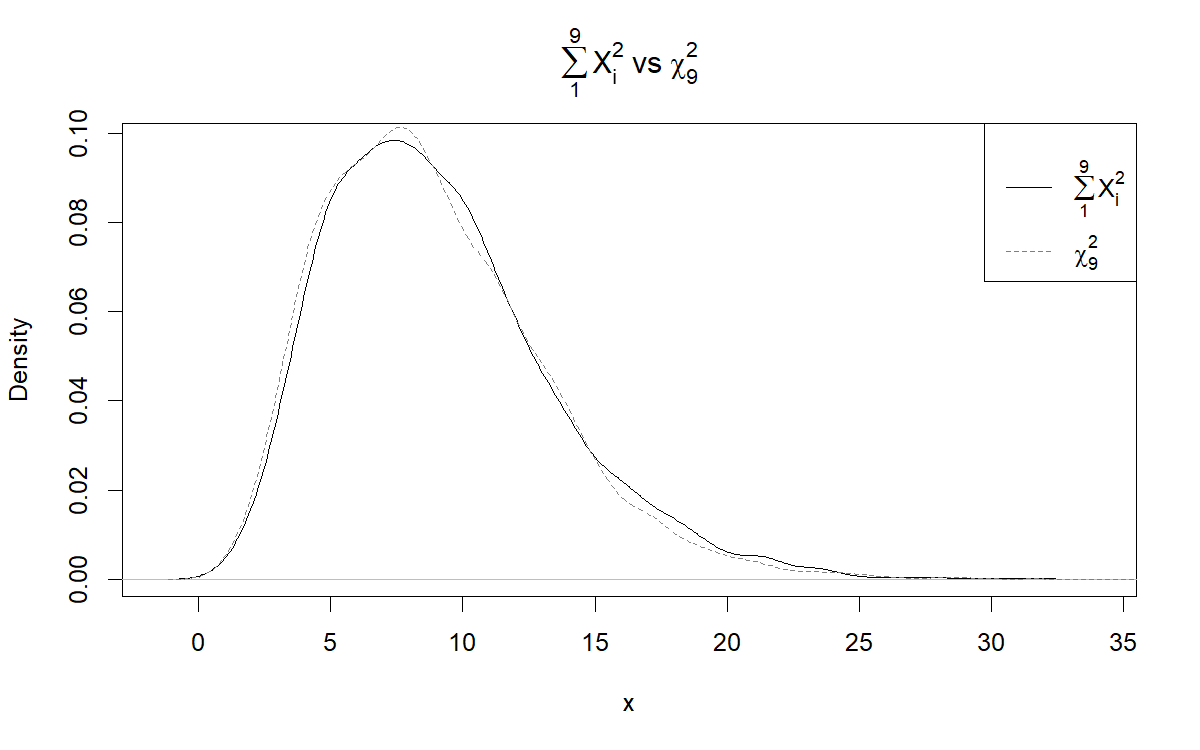
\includegraphics[width=0.6\textwidth]{Images/7a.png}
            \end{center}
        \end{soln}
    \end{subprob}

    \newpage

    \begin{subprob}
        The empirical distribution of $3 \bar{X} / S$ (using a solid line) is close to that of $t_8$ (using a dashed line), where $X_i \sim \text{i.i.d.} N (0, 1)$, $\bar{X} = \frac{1}{9} \sum_{i=1}^9 X_i$, and $S^2 = \frac{1}{8} \sum_{i=1}^9 (X_i - \bar{X})^2$.

        \begin{verbatim}
set.seed(42)
n_rep <- 5000

png("7b.png", width = 8, height = 5, units = "in", res = 150)  # landscape

empirical <- replicate(n_rep, {
  x <- rnorm(9, 0, 1)
  3 * mean(x) / sqrt((1 / 8) * sum((x - mean(x))^2))
})

theoretical <- rt(n_rep, df = 8)

dens_emp <- density(empirical)
dens_theo <- density(theoretical)

plot(dens_emp, type = "l", lty = 1, col = "black",
        xlab = "x", ylab = "Density",
        main = expression(3 * bar(X) / S ~ "vs" ~ t[8]))
lines(dens_theo, lty = 2, col = "gray50")
legend("topright",
        legend = c(expression(3 * bar(X) / S), expression(t[8])),
        lty = c(1, 2), col = c("black", "gray50"))

dev.off()            
        \end{verbatim}

        \begin{soln}
            \begin{center}
                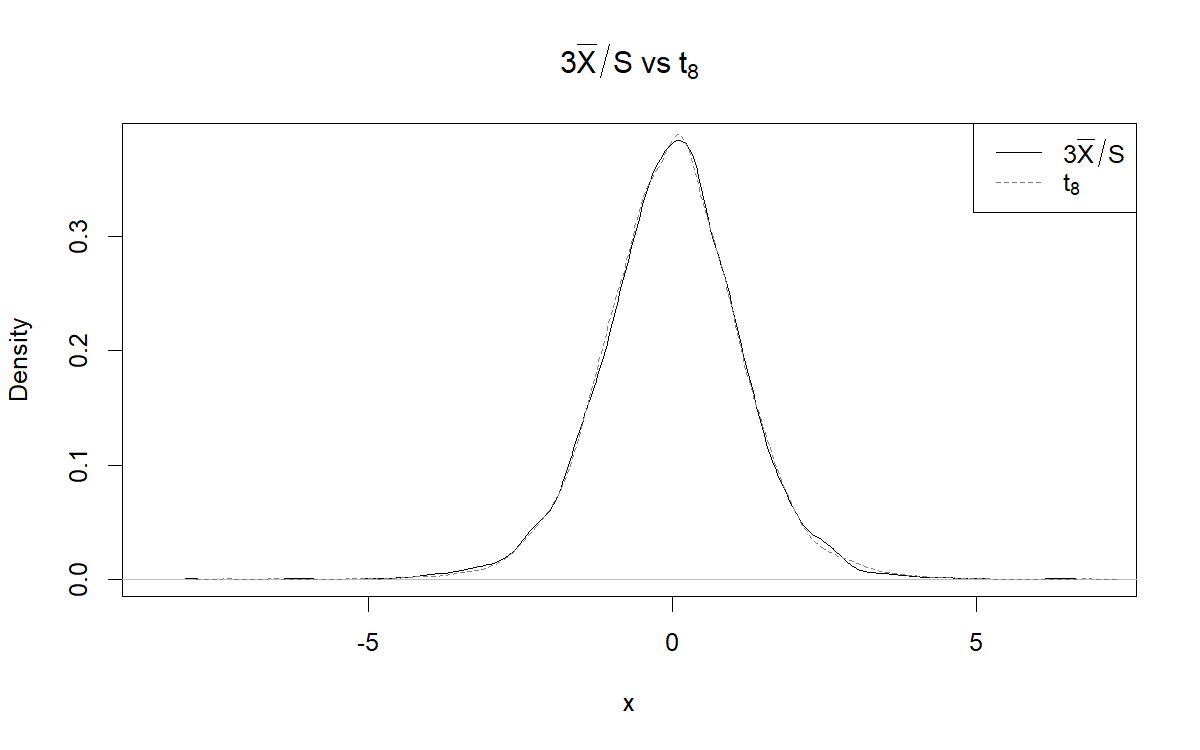
\includegraphics[width=0.6\textwidth]{Images/7b.png}
            \end{center}
        \end{soln}
    \end{subprob}
    \end{subprobset}
\end{prob}
\end{probset}
\end{document}